\documentclass[]{article}

\usepackage{amsmath}
\usepackage{amsfonts}
\usepackage{amsthm}
\usepackage{amssymb}
\usepackage{mathrsfs}
\usepackage{stmaryrd}
\usepackage{tikz}
\usepackage{hyperref}

\newcommand{\Q}{\mathbb{Q}}
\newcommand{\N}{\mathbb{N}}
\newcommand{\Z}{\mathbb{Z}}
\newcommand{\R}{\mathbb{R}}
\newcommand{\E}{\mathbb{E}}
\newcommand{\Var}{\mathrm{Var}}
\newcommand{\Cov}{\mathrm{Cov}}
\newcommand{\Primes}{\mathbb{P}}
\newcommand{\st}{\text{ s.t. }}
\newcommand{\txtand}{\text{ and }}
\newcommand{\txtor}{\text{ or }}
\newcommand{\lxor}{\veebar}
\newcommand{\Ito}{It\^{o}}
\newcommand{\dd}{\mathrm{d}}

%opening
\title{Notes on \Ito{} Calculus}
\author{DSBA Mathematics Refresher 2026}
\date{}

\begin{document}

	\maketitle

	\begin{abstract}
		This session is \textbf{optional}, and meant to be done \textbf{from home, autonomously}: there is no class, and no professor to ask.
		Everything you need is in these notes, and every exercise of the problem set comes with a full written solution.
		It is a bonus session: it does \textit{not} count towards the validation of the course.

		The goal is to give you a first, honest feel for \textbf{stochastic calculus} (calculus applied to functions that are random and nowhere smooth).
		In particular for \Ito's lemma, the chain rule of the random world.
		This is the mathematical language of quantitative finance, of diffusion models in machine learning, and of a good part of continuous-time modelling in general.
		It builds directly on session on Calculus and session on Differential Equations.

	\end{abstract}

	\tableofcontents

	\section{Why Another Calculus?}

	\subsection{The Problem}

	In Session 7 we modelled a customer base with the differential equation
	$$
	\frac{dN}{dt} = a - b\,N
	$$
	and we solved it exactly: $N(t) = \frac{a}{b} + \left(N_0 - \frac{a}{b}\right)e^{-bt}$.
	The model is \textbf{deterministic}: given $N_0$, and one can tell $N(t)$ for every future $t$, to the last decimal.

	A company does not acquire exactly $500$ customers every month; a stock price does not follow a smooth curve; a queue does not fill up at a constant rate.
	Real dynamic systems have a \textit{trend} \textbf{and} a \textit{noise}, and the noise does not average away.
	
	The natural thing to write down is therefore something like
	$$
	\frac{dX}{dt} = \underbrace{\mu(t, X_t)}_{\text{trend}} + \underbrace{\sigma(t, X_t) \cdot \xi_t}_{\text{noise}}
	$$
	where $\xi_t$ is "random noise at time $t$''.
	This looks harmless. It is not: it turns out that no reasonable function $\xi_t$ does what we want, and that the object $\frac{dX}{dt}$ does not exist for the processes we care about.
	The whole point of \Ito{} calculus is to make sense of this equation anyway.
	The idea is to never divide by $dt$, and write it in \textbf{differential} form instead:
	$$
	\boxed{\;\dd X_t = \mu(t, X_t)\, \dd t + \sigma(t, X_t)\, \dd W_t\;}
	$$
	where $W_t$ is Brownian motion, the object of the next section.
	This is a \textbf{stochastic differential equation} (SDE).
	The rest of these notes explains what each symbol means, and how to compute with them.

	\subsection{Where It Is Used}

	\paragraph{Quantitative finance.}
	The standard model of a stock price is \textbf{geometric Brownian motion}, $\dd S_t = \mu S_t \dd t + \sigma S_t \dd W_t$, and the Black--Scholes option pricing formula is derived in three lines of \Ito{} calculus (Section~7).
	Interest rate models (Vasicek, Cox--Ingersoll--Ross, Hull--White) are all SDEs.

	\paragraph{Machine learning.}
	\textbf{Diffusion models} (Stable Diffusion, DALL$\cdot$E, and the whole family of modern image and video generators) are literally built on an SDE: the forward process gradually adds Gaussian noise to an image, and the model learns to run the corresponding \textit{reverse-time} SDE.
	\textbf{Stochastic gradient descent} itself is often analysed as a discretisation of an SDE, which is how people explain why the noise in SGD helps it escape sharp minima.

	\paragraph{Elsewhere.}
	Population dynamics with random environment, chemical reaction networks, queueing systems under heavy traffic, filtering (the Kalman--Bucy filter), and physical Brownian motion itself, the historical origin of the whole subject.

	\section{Brownian Motion}

	\subsection{From a Random Walk}

	Start with something completely elementary.
	Let $Z_1, Z_2, \dots$ be independent coin flips, $Z_i = \pm 1$ with probability $\frac12$ each, and let
	$$
	S_n = Z_1 + Z_2 + \dots + Z_n
	$$
	be the position after $n$ steps of a \textbf{random walk}.
	We know that $\E[S_n] = 0$ and, since the $Z_i$ are independent, $\Var(S_n) = n$.
	So the walk drifts nowhere on average, but it spreads out: after $n$ steps it is typically at distance $\sqrt{n}$ from the origin.

	Now speed the walk up and shrink the steps.
	Fix a time horizon $t$, cut $[0,t]$ into $n$ intervals of length $\frac{t}{n}$, and take a step of size $\sqrt{t/n}$ at each of them:
	$$
	W^{(n)}_t = \sqrt{\frac{t}{n}} \; \big(Z_1 + \dots + Z_n\big)
	$$
	Then $\E[W^{(n)}_t] = 0$ and $\Var(W^{(n)}_t) = \frac{t}{n} \cdot n = t$, \textit{for every $n$}.
	The scaling $\sqrt{t/n}$ is the only one that keeps the variance finite and non-zero, and this is the first hint that in this world, \textbf{time scales like the square of space}.
	By the Central Limit Theorem, as $n \to \infty$,
	$$
	W^{(n)}_t \; \longrightarrow \; \mathcal{N}(0, t)
	$$
	The limiting object, as a function of $t$, is \textbf{Brownian motion} (or the \textbf{Wiener process}) $W_t$.

	\begin{center}
		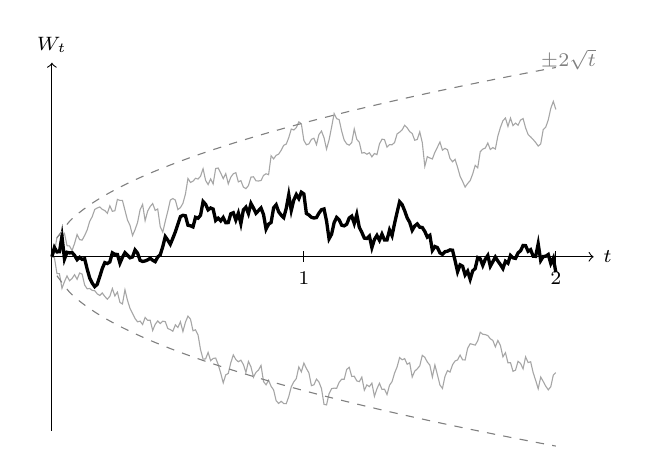
\begin{tikzpicture}[xscale=3.2,yscale=0.85]
			\draw[->] (0,0) -- (2.15,0) node[right] {\scriptsize $t$};
			\draw[->] (0,-2.6) -- (0,2.9) node[above] {\scriptsize $W_t$};
			\draw (1,0.08) -- (1,-0.08) node[below] {\scriptsize $1$};
			\draw (2,0.08) -- (2,-0.08) node[below] {\scriptsize $2$};
			\draw[gray!70] (0.000,0.000) -- (0.010,-0.012) -- (0.020,-0.250) -- (0.030,-0.253) -- (0.040,-0.472) -- (0.050,-0.371) -- (0.060,-0.286) -- (0.070,-0.358) -- (0.080,-0.325) -- (0.090,-0.268) -- (0.100,-0.337) -- (0.110,-0.243) -- (0.120,-0.259) -- (0.130,-0.422) -- (0.140,-0.479) -- (0.150,-0.473) -- (0.160,-0.502) -- (0.170,-0.507) -- (0.180,-0.554) -- (0.190,-0.578) -- (0.200,-0.541) -- (0.210,-0.593) -- (0.220,-0.634) -- (0.230,-0.590) -- (0.240,-0.475) -- (0.250,-0.585) -- (0.260,-0.528) -- (0.270,-0.682) -- (0.280,-0.705) -- (0.290,-0.493) -- (0.300,-0.651) -- (0.310,-0.770) -- (0.320,-0.845) -- (0.330,-0.922) -- (0.340,-0.972) -- (0.350,-0.961) -- (0.360,-1.012) -- (0.370,-0.906) -- (0.380,-0.949) -- (0.390,-0.947) -- (0.400,-1.101) -- (0.410,-1.009) -- (0.420,-0.959) -- (0.430,-0.997) -- (0.440,-0.963) -- (0.450,-0.969) -- (0.460,-1.072) -- (0.470,-1.088) -- (0.480,-1.113) -- (0.490,-1.017) -- (0.500,-1.057) -- (0.510,-0.971) -- (0.520,-1.117) -- (0.530,-0.977) -- (0.540,-0.887) -- (0.550,-0.931) -- (0.560,-1.106) -- (0.570,-1.091) -- (0.580,-1.167) -- (0.590,-1.389) -- (0.600,-1.530) -- (0.610,-1.526) -- (0.620,-1.429) -- (0.630,-1.552) -- (0.640,-1.519) -- (0.650,-1.513) -- (0.660,-1.610) -- (0.670,-1.738) -- (0.680,-1.884) -- (0.690,-1.764) -- (0.700,-1.743) -- (0.710,-1.583) -- (0.720,-1.467) -- (0.730,-1.535) -- (0.740,-1.569) -- (0.750,-1.545) -- (0.760,-1.610) -- (0.770,-1.729) -- (0.780,-1.564) -- (0.790,-1.644) -- (0.800,-1.799) -- (0.810,-1.726) -- (0.820,-1.692) -- (0.830,-1.623) -- (0.840,-1.866) -- (0.850,-1.913) -- (0.860,-1.845) -- (0.870,-1.936) -- (0.880,-1.990) -- (0.890,-2.152) -- (0.900,-2.191) -- (0.910,-2.159) -- (0.920,-2.193) -- (0.930,-2.195) -- (0.940,-2.090) -- (0.950,-1.942) -- (0.960,-1.869) -- (0.970,-1.819) -- (0.980,-1.646) -- (0.990,-1.720) -- (1.000,-1.589) -- (1.010,-1.668) -- (1.020,-1.735) -- (1.030,-1.925) -- (1.040,-1.913) -- (1.050,-1.828) -- (1.060,-1.872) -- (1.070,-1.970) -- (1.080,-2.205) -- (1.090,-2.213) -- (1.100,-2.046) -- (1.110,-1.970) -- (1.120,-1.963) -- (1.130,-1.966) -- (1.140,-1.876) -- (1.150,-1.829) -- (1.160,-1.831) -- (1.170,-1.683) -- (1.180,-1.651) -- (1.190,-1.788) -- (1.200,-1.785) -- (1.210,-1.854) -- (1.220,-1.866) -- (1.230,-1.798) -- (1.240,-1.994) -- (1.250,-1.915) -- (1.260,-1.940) -- (1.270,-1.888) -- (1.280,-2.085) -- (1.290,-1.972) -- (1.300,-1.890) -- (1.310,-1.982) -- (1.320,-1.978) -- (1.330,-2.059) -- (1.340,-1.919) -- (1.350,-1.865) -- (1.360,-1.738) -- (1.370,-1.646) -- (1.380,-1.506) -- (1.390,-1.539) -- (1.400,-1.522) -- (1.410,-1.606) -- (1.420,-1.584) -- (1.430,-1.797) -- (1.440,-1.709) -- (1.450,-1.675) -- (1.460,-1.629) -- (1.470,-1.472) -- (1.480,-1.502) -- (1.490,-1.573) -- (1.500,-1.619) -- (1.510,-1.798) -- (1.520,-1.617) -- (1.530,-1.762) -- (1.540,-1.915) -- (1.550,-1.967) -- (1.560,-1.788) -- (1.570,-1.700) -- (1.580,-1.723) -- (1.590,-1.614) -- (1.600,-1.558) -- (1.610,-1.541) -- (1.620,-1.469) -- (1.630,-1.539) -- (1.640,-1.542) -- (1.650,-1.367) -- (1.660,-1.299) -- (1.670,-1.309) -- (1.680,-1.320) -- (1.690,-1.256) -- (1.700,-1.128) -- (1.710,-1.157) -- (1.720,-1.163) -- (1.730,-1.177) -- (1.740,-1.225) -- (1.750,-1.250) -- (1.760,-1.346) -- (1.770,-1.251) -- (1.780,-1.325) -- (1.790,-1.495) -- (1.800,-1.433) -- (1.810,-1.585) -- (1.820,-1.581) -- (1.830,-1.711) -- (1.840,-1.694) -- (1.850,-1.562) -- (1.860,-1.594) -- (1.870,-1.674) -- (1.880,-1.495) -- (1.890,-1.581) -- (1.900,-1.568) -- (1.910,-1.732) -- (1.920,-1.846) -- (1.930,-1.972) -- (1.940,-1.797) -- (1.950,-1.863) -- (1.960,-1.934) -- (1.970,-1.988) -- (1.980,-1.941) -- (1.990,-1.767) -- (2.000,-1.731);
			\draw[gray!70] (0.000,0.000) -- (0.010,0.061) -- (0.020,0.288) -- (0.030,0.327) -- (0.040,0.295) -- (0.050,0.347) -- (0.060,0.166) -- (0.070,0.161) -- (0.080,0.093) -- (0.090,0.200) -- (0.100,0.333) -- (0.110,0.256) -- (0.120,0.249) -- (0.130,0.318) -- (0.140,0.401) -- (0.150,0.529) -- (0.160,0.599) -- (0.170,0.707) -- (0.180,0.729) -- (0.190,0.744) -- (0.200,0.708) -- (0.210,0.691) -- (0.220,0.650) -- (0.230,0.761) -- (0.240,0.679) -- (0.250,0.688) -- (0.260,0.857) -- (0.270,0.842) -- (0.280,0.843) -- (0.290,0.694) -- (0.300,0.549) -- (0.310,0.469) -- (0.320,0.317) -- (0.330,0.405) -- (0.340,0.512) -- (0.350,0.702) -- (0.360,0.783) -- (0.370,0.539) -- (0.380,0.682) -- (0.390,0.750) -- (0.400,0.795) -- (0.410,0.693) -- (0.420,0.714) -- (0.430,0.449) -- (0.440,0.367) -- (0.450,0.531) -- (0.460,0.681) -- (0.470,0.847) -- (0.480,0.870) -- (0.490,0.847) -- (0.500,0.705) -- (0.510,0.734) -- (0.520,0.798) -- (0.530,0.937) -- (0.540,1.170) -- (0.550,1.111) -- (0.560,1.129) -- (0.570,1.173) -- (0.580,1.161) -- (0.590,1.204) -- (0.600,1.315) -- (0.610,1.142) -- (0.620,1.079) -- (0.630,1.163) -- (0.640,1.088) -- (0.650,1.319) -- (0.660,1.326) -- (0.670,1.252) -- (0.680,1.168) -- (0.690,1.243) -- (0.700,1.089) -- (0.710,1.189) -- (0.720,1.240) -- (0.730,1.257) -- (0.740,1.119) -- (0.750,1.138) -- (0.760,1.041) -- (0.770,1.018) -- (0.780,1.064) -- (0.790,1.190) -- (0.800,1.195) -- (0.810,1.135) -- (0.820,1.132) -- (0.830,1.140) -- (0.840,1.216) -- (0.850,1.240) -- (0.860,1.226) -- (0.870,1.509) -- (0.880,1.463) -- (0.890,1.516) -- (0.900,1.534) -- (0.910,1.591) -- (0.920,1.665) -- (0.930,1.683) -- (0.940,1.779) -- (0.950,1.908) -- (0.960,1.895) -- (0.970,1.930) -- (0.980,2.016) -- (0.990,1.987) -- (1.000,1.739) -- (1.010,1.673) -- (1.020,1.687) -- (1.030,1.755) -- (1.040,1.771) -- (1.050,1.675) -- (1.060,1.827) -- (1.070,1.878) -- (1.080,1.778) -- (1.090,1.608) -- (1.100,1.746) -- (1.110,1.936) -- (1.120,2.139) -- (1.130,2.064) -- (1.140,2.049) -- (1.150,1.878) -- (1.160,1.743) -- (1.170,1.686) -- (1.180,1.668) -- (1.190,1.707) -- (1.200,1.910) -- (1.210,1.755) -- (1.220,1.711) -- (1.230,1.549) -- (1.240,1.557) -- (1.250,1.532) -- (1.260,1.554) -- (1.270,1.493) -- (1.280,1.543) -- (1.290,1.526) -- (1.300,1.685) -- (1.310,1.757) -- (1.320,1.751) -- (1.330,1.638) -- (1.340,1.675) -- (1.350,1.674) -- (1.360,1.707) -- (1.370,1.836) -- (1.380,1.862) -- (1.390,1.896) -- (1.400,1.965) -- (1.410,1.927) -- (1.420,1.870) -- (1.430,1.842) -- (1.440,1.741) -- (1.450,1.753) -- (1.460,1.866) -- (1.470,1.706) -- (1.480,1.351) -- (1.490,1.496) -- (1.500,1.476) -- (1.510,1.461) -- (1.520,1.562) -- (1.530,1.637) -- (1.540,1.715) -- (1.550,1.593) -- (1.560,1.620) -- (1.570,1.600) -- (1.580,1.468) -- (1.590,1.420) -- (1.600,1.457) -- (1.610,1.338) -- (1.620,1.204) -- (1.630,1.126) -- (1.640,1.041) -- (1.650,1.095) -- (1.660,1.137) -- (1.670,1.237) -- (1.680,1.366) -- (1.690,1.329) -- (1.700,1.569) -- (1.710,1.608) -- (1.720,1.624) -- (1.730,1.699) -- (1.740,1.603) -- (1.750,1.631) -- (1.760,1.610) -- (1.770,1.805) -- (1.780,1.932) -- (1.790,2.033) -- (1.800,2.073) -- (1.810,1.948) -- (1.820,2.072) -- (1.830,1.961) -- (1.840,1.997) -- (1.850,1.966) -- (1.860,2.042) -- (1.870,2.065) -- (1.880,1.926) -- (1.890,1.826) -- (1.900,1.791) -- (1.910,1.752) -- (1.920,1.707) -- (1.930,1.654) -- (1.940,1.685) -- (1.950,1.901) -- (1.960,1.937) -- (1.970,2.046) -- (1.980,2.217) -- (1.990,2.322) -- (2.000,2.201);
			\draw[very thick] (0.000,0.000) -- (0.010,0.139) -- (0.020,0.073) -- (0.030,0.075) -- (0.040,0.305) -- (0.050,-0.033) -- (0.060,0.067) -- (0.070,0.057) -- (0.080,0.063) -- (0.090,0.021) -- (0.100,-0.043) -- (0.110,-0.008) -- (0.120,-0.039) -- (0.130,-0.029) -- (0.140,-0.184) -- (0.150,-0.316) -- (0.160,-0.394) -- (0.170,-0.446) -- (0.180,-0.411) -- (0.190,-0.296) -- (0.200,-0.175) -- (0.210,-0.087) -- (0.220,-0.101) -- (0.230,-0.076) -- (0.240,0.059) -- (0.250,0.036) -- (0.260,0.035) -- (0.270,-0.095) -- (0.280,-0.007) -- (0.290,0.061) -- (0.300,0.025) -- (0.310,-0.015) -- (0.320,-0.002) -- (0.330,0.101) -- (0.340,0.054) -- (0.350,-0.053) -- (0.360,-0.070) -- (0.370,-0.062) -- (0.380,-0.047) -- (0.390,-0.023) -- (0.400,-0.052) -- (0.410,-0.073) -- (0.420,-0.004) -- (0.430,0.030) -- (0.440,0.151) -- (0.450,0.301) -- (0.460,0.248) -- (0.470,0.187) -- (0.480,0.277) -- (0.490,0.373) -- (0.500,0.487) -- (0.510,0.600) -- (0.520,0.620) -- (0.530,0.612) -- (0.540,0.471) -- (0.550,0.463) -- (0.560,0.446) -- (0.570,0.590) -- (0.580,0.576) -- (0.590,0.621) -- (0.600,0.825) -- (0.610,0.784) -- (0.620,0.701) -- (0.630,0.729) -- (0.640,0.713) -- (0.650,0.543) -- (0.660,0.577) -- (0.670,0.537) -- (0.680,0.587) -- (0.690,0.509) -- (0.700,0.511) -- (0.710,0.642) -- (0.720,0.658) -- (0.730,0.549) -- (0.740,0.652) -- (0.750,0.495) -- (0.760,0.701) -- (0.770,0.741) -- (0.780,0.646) -- (0.790,0.797) -- (0.800,0.728) -- (0.810,0.650) -- (0.820,0.690) -- (0.830,0.729) -- (0.840,0.630) -- (0.850,0.413) -- (0.860,0.488) -- (0.870,0.513) -- (0.880,0.732) -- (0.890,0.777) -- (0.900,0.672) -- (0.910,0.622) -- (0.920,0.585) -- (0.930,0.722) -- (0.940,0.926) -- (0.950,0.692) -- (0.960,0.847) -- (0.970,0.930) -- (0.980,0.869) -- (0.990,0.965) -- (1.000,0.939) -- (1.010,0.647) -- (1.020,0.625) -- (1.030,0.590) -- (1.040,0.579) -- (1.050,0.586) -- (1.060,0.653) -- (1.070,0.703) -- (1.080,0.714) -- (1.090,0.534) -- (1.100,0.269) -- (1.110,0.337) -- (1.120,0.508) -- (1.130,0.588) -- (1.140,0.553) -- (1.150,0.472) -- (1.160,0.462) -- (1.170,0.486) -- (1.180,0.579) -- (1.190,0.607) -- (1.200,0.498) -- (1.210,0.633) -- (1.220,0.440) -- (1.230,0.365) -- (1.240,0.279) -- (1.250,0.273) -- (1.260,0.310) -- (1.270,0.137) -- (1.280,0.258) -- (1.290,0.319) -- (1.300,0.247) -- (1.310,0.338) -- (1.320,0.251) -- (1.330,0.251) -- (1.340,0.400) -- (1.350,0.316) -- (1.360,0.499) -- (1.370,0.664) -- (1.380,0.822) -- (1.390,0.779) -- (1.400,0.688) -- (1.410,0.582) -- (1.420,0.515) -- (1.430,0.396) -- (1.440,0.460) -- (1.450,0.491) -- (1.460,0.441) -- (1.470,0.438) -- (1.480,0.378) -- (1.490,0.294) -- (1.500,0.320) -- (1.510,0.096) -- (1.520,0.153) -- (1.530,0.137) -- (1.540,0.058) -- (1.550,0.036) -- (1.560,0.076) -- (1.570,0.083) -- (1.580,0.103) -- (1.590,0.098) -- (1.600,-0.056) -- (1.610,-0.223) -- (1.620,-0.121) -- (1.630,-0.141) -- (1.640,-0.271) -- (1.650,-0.215) -- (1.660,-0.336) -- (1.670,-0.211) -- (1.680,-0.175) -- (1.690,-0.012) -- (1.700,-0.030) -- (1.710,-0.129) -- (1.720,-0.037) -- (1.730,0.019) -- (1.740,-0.141) -- (1.750,-0.073) -- (1.760,-0.004) -- (1.770,-0.064) -- (1.780,-0.117) -- (1.790,-0.176) -- (1.800,-0.067) -- (1.810,-0.096) -- (1.820,0.020) -- (1.830,-0.016) -- (1.840,-0.024) -- (1.850,0.058) -- (1.860,0.089) -- (1.870,0.169) -- (1.880,0.166) -- (1.890,0.082) -- (1.900,0.106) -- (1.910,0.009) -- (1.920,0.006) -- (1.930,0.194) -- (1.940,-0.056) -- (1.950,0.004) -- (1.960,0.008) -- (1.970,0.034) -- (1.980,-0.100) -- (1.990,-0.019) -- (2.000,-0.231);
			% variance envelope
			\draw[dashed,gray,domain=0.02:2,samples=40,smooth] plot ({\x},{2*sqrt(\x)});
			\draw[dashed,gray,domain=0.02:2,samples=40,smooth] plot ({\x},{-2*sqrt(\x)});
			\node[gray] at (2.05,2.95) {\scriptsize $\pm 2\sqrt{t}$};
		\end{tikzpicture}
	\end{center}
	Three sample paths of Brownian motion. The dashed curves are $\pm 2\sqrt{t}$: the paths spread out like the \textit{square root} of time, not like time.

	\subsection{Definition and Properties}

	\textbf{Definition.} A \textbf{standard Brownian motion} is a family of random variables $(W_t)_{t \geq 0}$ such that:
	\begin{enumerate}
		\item $W_0 = 0$;
		\item \textbf{independent increments}: for $0 \leq s < t \leq u < v$, the increments $W_t - W_s$ and $W_v - W_u$ are independent;
		\item \textbf{Gaussian increments}: for $s < t$, \quad $W_t - W_s \sim \mathcal{N}(0, \, t - s)$;
		\item the map $t \mapsto W_t$ is \textbf{continuous}.
	\end{enumerate}

	It is a genuine theorem (Wiener, 1923) that such an object exists, as it is not obvious that conditions 2--4 are compatible.

	From the definition, three computations that you will use constantly:
	$$
	\E[W_t] = 0, \qquad \Var(W_t) = \E[W_t^2] = t, \qquad \Cov(W_s, W_t) = \min(s,t)
	$$
	The last one is worth doing once: for $s < t$, write $W_t = W_s + (W_t - W_s)$; the second term is independent of $W_s$ and has mean $0$, so
	$$
	\Cov(W_s, W_t) = \E[W_s W_t] = \E[W_s^2] + \E[W_s]\,\E[W_t - W_s] = s + 0 = s = \min(s,t)
	$$

	\subsection{The Paths}

	Here is the crucial point, the one that forces us to build a new calculus.
	The paths $t \mapsto W_t$ are continuous, but:

	\paragraph{They are nowhere differentiable.}
	Consider the difference quotient over a small interval $h$:
	$$
	\frac{W_{t+h} - W_t}{h} \sim \frac{\mathcal{N}(0,h)}{h} = \mathcal{N}\!\left(0, \frac{1}{h}\right)
	$$
	using $\Var(cX) = c^2\Var(X)$ with $c = 1/h$.
	As $h \to 0$, the variance $\frac{1}{h}$ blows up: the quotient does not settle down to anything.
	With probability $1$, a Brownian path has \textbf{no derivative at any point}.
	So $\frac{dW}{dt}$ (the "noise'' $\xi_t$ of Section 1.1) simply does not exist, and $\frac{dX}{dt} = \mu + \sigma \xi_t$ is meaningless as written.

	\paragraph{They have infinite length.}
	A Brownian path has infinite total variation on any interval: it wiggles so much that if you tried to measure its length with a piece of string, you would need infinitely much string.
	This kills the standard (Riemann--Stieltjes) way of defining an integral $\int f \, dg$, which requires $g$ to have finite variation.

	\paragraph{But their \textit{quadratic} variation is finite, and deterministic.}
	This is the miracle that saves everything.
	Cut $[0,T]$ into $n$ pieces $0 = t_0 < t_1 < \dots < t_n = T$ of length $\Delta t = \frac{T}{n}$, and instead of summing the increments, sum their \textbf{squares}:
	$$
	Q_n = \sum_{i=1}^{n} \left(W_{t_i} - W_{t_{i-1}}\right)^2
	$$
	Each increment is $\mathcal{N}(0, \Delta t)$, so each square has expectation $\Delta t$, and
	$$
	\E[Q_n] = \sum_{i=1}^n \Delta t = n \cdot \frac{T}{n} = T
	$$
	More interestingly, the variance vanishes. For $Z \sim \mathcal{N}(0,\Delta t)$ one has $\Var(Z^2) = 2(\Delta t)^2$, and the $n$ terms are independent, so
	$$
	\Var(Q_n) = n \cdot 2 \left(\frac{T}{n}\right)^2 = \frac{2T^2}{n} \; \xrightarrow[n \to \infty]{} \; 0
	$$
	So $Q_n \to T$, \textbf{and not merely on average}: the randomness disappears in the limit.

	\textbf{The quadratic variation of Brownian motion over $[0,T]$ is $T$, with probability 1.}

	Compare with a smooth function $f$: there $|f(t_i) - f(t_{i-1})| \approx |f'| \Delta t$, the squares are of size $(\Delta t)^2$, and the sum of $n$ of them is of order $n (\Delta t)^2 = T^2/n \to 0$.
	A smooth function has \textbf{zero} quadratic variation. Brownian motion does not. That single fact is the whole difference between the two calculi.

	\section{The Rule $(\dd W)^2 = \dd t$}

	The result above is usually written in the compact, deliberately informal form
	$$
	\boxed{\;(\dd W_t)^2 = \dd t\;}
	$$
	which is to be read as: "when you sum up squared Brownian increments, they behave like $\dd t$, not like something negligible''.
	Together with it come
	$$
	\dd t \cdot \dd t = 0, \qquad \dd t \cdot \dd W_t = 0
	$$
	(the first because $(\Delta t)^2$ summed $n$ times vanishes, as we just saw; the second for a similar reason).
	It is convenient to remember these as a multiplication table:
	$$
	\begin{array}{c|cc}
		\times & \dd t & \dd W_t \\
		\hline
		\dd t & 0 & 0 \\
		\dd W_t & 0 & \dd t
	\end{array}
	$$

	The intuition to keep: an increment of $W$ over a time $\dd t$ has size $\sqrt{\dd t}$.
	And $\sqrt{\dd t}$ is much \textit{bigger} than $\dd t$ when $\dd t$ is small ($\sqrt{0.0001} = 0.01 \gg 0.0001$).
	So terms which are "second order'' in the deterministic world are \textbf{first order} here, and cannot be thrown away.
	That is the entire content of \Ito{} calculus.

	\section{The \Ito{} Integral}

	Since $\frac{dW}{dt}$ does not exist, the only way to give meaning to $\dd X_t = \mu \dd t + \sigma \dd W_t$ is to declare it a shorthand for the \textbf{integral} statement
	$$
	X_T = X_0 + \int_0^T \mu(t, X_t) \, \dd t + \int_0^T \sigma(t, X_t) \, \dd W_t
	$$
	The first integral is an ordinary one. The second is new, and we must define it.

	\subsection{Definition}

	For a process $H_t$ (the \textbf{integrand}), define
	$$
	\int_0^T H_t \, \dd W_t = \lim_{n \to \infty} \sum_{i=1}^{n} H_{t_{i-1}} \left(W_{t_i} - W_{t_{i-1}}\right)
	$$
	This looks like a Riemann sum, and it is, with one absolutely essential difference.

	\paragraph{The evaluation point matters.}
	In ordinary calculus, $\int_a^b f \, dg$ can be approximated by evaluating $f$ at the left end, the right end, or the middle of each subinterval: the limit is the same.
	Here it is \textbf{not}.
	Because the increment $W_{t_i} - W_{t_{i-1}}$ has size $\sqrt{\Delta t}$ and not $\Delta t$, the choice of evaluation point changes the answer by a finite amount (Exercise 4 of the problem set makes this explicit).

	\Ito's choice is the \textbf{left endpoint} $t_{i-1}$, and it is not an arbitrary convention.
	It means the integrand is evaluated \textit{before} the increment it multiplies is revealed, so the process $H$ is \textbf{non-anticipating}.
	In finance this is exactly the statement that you must choose your portfolio \textit{before} you observe tomorrow's price move; a rule evaluating at the right endpoint would let you trade on information you do not have, and would price away all risk.

	(The mid-point choice gives a different, also useful, object: the \textbf{Stratonovich integral}, written $\int H \circ \dd W$. It obeys the ordinary chain rule, but it is anticipating, and is preferred in physics rather than in finance.)

	\subsection{The Two Properties You Need}

	\paragraph{1. Zero mean (martingale property).}
	$$
	\E\left[\int_0^T H_t \, \dd W_t\right] = 0
	$$
	\textit{Why:} in each term of the sum, $H_{t_{i-1}}$ is known at time $t_{i-1}$ while the increment $W_{t_i} - W_{t_{i-1}}$ is independent of the past and has mean $0$; so each term has expectation $\E[H_{t_{i-1}}] \cdot 0 = 0$.
	This is precisely where the left-endpoint choice is used (with the right endpoint, $H_{t_i}$ and the increment would be correlated, and the mean would not vanish).

	Consequently the process $t \mapsto \int_0^t H_s \dd W_s$ is a \textbf{martingale}: its best forecast for any future date is its present value.
	"Driftless'' and "$\dd t$-free'' are the same thing.

	\paragraph{2. \Ito{} isometry.}
	$$
	\E\left[\left(\int_0^T H_t \, \dd W_t\right)^{\!2}\right] = \E\left[\int_0^T H_t^2 \, \dd t\right]
	$$
	This converts a variance of a stochastic integral into an ordinary integral, and it is the workhorse for every variance computation.
	\textit{Why:} expand the square of the sum. The cross terms $H_{t_{i-1}}H_{t_{j-1}}\Delta W_i \Delta W_j$ ($i \neq j$) have mean $0$ by independence of increments; the diagonal terms give $\E[H_{t_{i-1}}^2] \cdot \E[(\Delta W_i)^2] = \E[H_{t_{i-1}}^2] \Delta t$, which is a Riemann sum for $\E\int_0^T H_t^2 \dd t$.

	\paragraph{Example.}
	$\int_0^T \dd W_t = W_T$, which indeed has mean $0$ and variance $\E[W_T^2] = T = \int_0^T 1^2 \dd t$. \checkmark

	\section{\Ito's Lemma}

	This is the central result of the session: the \textbf{chain rule} of stochastic calculus.

	\subsection{Statement}

	Let $X_t$ satisfy the SDE
	$$
	\dd X_t = \mu_t \, \dd t + \sigma_t \, \dd W_t
	$$
	and let $f(t,x)$ be a function, twice differentiable in $x$ and once in $t$. Then $Y_t = f(t, X_t)$ is itself an \Ito{} process, and
	$$
	\boxed{\;
	\dd f(t,X_t) = \left(\frac{\partial f}{\partial t} + \mu_t \frac{\partial f}{\partial x} + \frac{1}{2}\sigma_t^2 \frac{\partial^2 f}{\partial x^2}\right) \dd t \; + \; \sigma_t \frac{\partial f}{\partial x} \, \dd W_t
	\;}
	$$
	all partial derivatives being evaluated at $(t, X_t)$.

	Compare with the ordinary chain rule, which for a smooth $x(t)$ would give $\dd f = \left(\partial_t f + \dot{x}\,\partial_x f\right)\dd t$.
	Everything is the same \textbf{except} the extra term
	$$
	\frac{1}{2}\sigma_t^2 \frac{\partial^2 f}{\partial x^2} \, \dd t
	$$
	called the \textbf{\Ito{} correction}. It is the entire novelty, and it is the reason random systems do not behave like their averages.

	\subsection{Where the Correction Comes From}

	Take the Taylor expansion of $f$ to second order:
	$$
	\dd f = \frac{\partial f}{\partial t} \dd t + \frac{\partial f}{\partial x} \dd X + \frac{1}{2}\frac{\partial^2 f}{\partial x^2} (\dd X)^2 + \frac{\partial^2 f}{\partial t \partial x}\dd t \, \dd X + \frac{1}{2}\frac{\partial^2 f}{\partial t^2}(\dd t)^2 + \dots
	$$
	In ordinary calculus, every term beyond the first order is negligible and we stop after two terms.
	Here we use the multiplication table of Section 3 on $(\dd X)^2$:
	$$
	(\dd X)^2 = \left(\mu \dd t + \sigma \dd W\right)^2 = \mu^2 \underbrace{(\dd t)^2}_{=\,0} + 2\mu\sigma \underbrace{\dd t \, \dd W}_{=\,0} + \sigma^2 \underbrace{(\dd W)^2}_{=\,\dd t} = \sigma^2 \dd t
	$$
	So the second-order term in $x$ is \textbf{of order $\dd t$}: it survives.
	The last two terms above are genuinely negligible ($\dd t \dd X$ and $(\dd t)^2$ are both $0$).
	Substituting $\dd X = \mu \dd t + \sigma \dd W$ and $(\dd X)^2 = \sigma^2 \dd t$ and collecting the $\dd t$ and $\dd W$ terms gives the boxed formula.

	That is genuinely all there is to it: \textbf{\Ito's lemma is a second-order Taylor expansion in which $(\dd W)^2$ has been replaced by $\dd t$.}

	\subsection{First Example: $f(x) = x^2$}

	Take $X_t = W_t$ itself (so $\mu = 0$, $\sigma = 1$) and $f(x) = x^2$, with $\partial_t f = 0$, $\partial_x f = 2x$, $\partial_{xx} f = 2$.
	\Ito's lemma gives
	$$
	\dd (W_t^2) = \left(0 + 0 \cdot 2W_t + \tfrac{1}{2}\cdot 1 \cdot 2\right)\dd t + 1 \cdot 2W_t \, \dd W_t = \dd t + 2 W_t \, \dd W_t
	$$
	Integrating from $0$ to $T$ (and using $W_0 = 0$) and rearranging:
	$$
	\int_0^T W_t \, \dd W_t = \frac{1}{2}W_T^2 - \frac{1}{2}T
	$$
	Look at this carefully. Ordinary calculus would have predicted $\int_0^T W \dd W = \frac12 W_T^2$, by analogy with $\int_0^T x \dd x = \frac12 x_T^2$.
	The extra $-\frac{T}{2}$ is the \Ito{} correction, and it is not a detail: without it the left-hand side would have mean $\E[\frac12 W_T^2] = \frac{T}{2} \neq 0$, contradicting the martingale property of Section 4.2.
	With it, $\E\left[\int_0^T W \dd W\right] = \frac{T}{2} - \frac{T}{2} = 0$. \checkmark

	\subsection{The Fundamental Example: Geometric Brownian Motion}

	Model a stock price by
	$$
	\dd S_t = \mu S_t \, \dd t + \sigma S_t \, \dd W_t
	$$
	i.e. \textit{relative} changes $\frac{\dd S_t}{S_t}$ have a constant trend $\mu$ (the expected return) and a constant noise level $\sigma$ (the volatility).
	This is \textbf{geometric Brownian motion} (GBM), the model underlying Black--Scholes.

	To solve it, apply \Ito's lemma to $f(x) = \ln x$, exactly as one would separate variables in the deterministic case.
	Here $\partial_t f = 0$, $\partial_x f = \frac{1}{x}$, $\partial_{xx} f = -\frac{1}{x^2}$, and with $\mu_t = \mu S_t$, $\sigma_t = \sigma S_t$:
	$$
	\dd (\ln S_t) = \left(\mu S_t \cdot \frac{1}{S_t} + \frac{1}{2}\sigma^2 S_t^2 \cdot \left(-\frac{1}{S_t^2}\right)\right)\dd t + \sigma S_t \cdot \frac{1}{S_t}\, \dd W_t
	$$
	$$
	= \left(\mu - \frac{\sigma^2}{2}\right)\dd t + \sigma \, \dd W_t
	$$
	The right-hand side no longer involves $S$, so we can integrate directly:
	$$
	\ln S_T - \ln S_0 = \left(\mu - \frac{\sigma^2}{2}\right)T + \sigma W_T
	$$
	$$
	\boxed{\;S_T = S_0 \exp\left(\left(\mu - \frac{\sigma^2}{2}\right)T + \sigma W_T\right)\;}
	$$

	Two things deserve comment.

	\paragraph{The $-\frac{\sigma^2}{2}$ is real money.}
	Naive integration of $\frac{\dd S}{S} = \mu \dd t + \sigma \dd W$ would give $S_T = S_0 e^{\mu T + \sigma W_T}$, without the correction.
	The difference is not cosmetic. Since $\E[e^{\sigma W_T}] = e^{\sigma^2 T/2}$ (the Gaussian moment generating function, with $W_T \sim \mathcal{N}(0,T)$), the correct formula gives
	$$
	\E[S_T] = S_0 e^{(\mu - \sigma^2/2)T} \cdot e^{\sigma^2 T /2} = S_0 e^{\mu T}
	$$
	which is what "expected return $\mu$'' ought to mean. The naive formula would give $S_0 e^{(\mu + \sigma^2/2)T}$: volatility would create free money out of nothing.

	\paragraph{Volatility drag.}
	The \textit{typical} path, on the other hand, grows like $e^{(\mu - \sigma^2/2)t}$, which is strictly less than $e^{\mu t}$.
	So if $\sigma^2 > 2\mu$, the asset has a positive expected value that grows forever, and yet almost every individual path tends to $0$.
	This is not a paradox (the mean is carried by rarer and rarer, larger and larger outcomes), and it is one of the most practically important consequences of \Ito's lemma.
	It is the mathematical content of the everyday observation that a $-50\%$ move followed by a $+50\%$ move leaves you down $25\%$.

	\section{Further Reading}

	If this session interested you, here are the three books to know.

	\begin{itemize}
		\item \textbf{Steven E. Shreve}, \textit{Stochastic Calculus for Finance I/II}, Springer, 2004.\\
		Written for readers with a solid calculus and probability background but no measure theory, it develops Brownian motion, the \Ito{} integral, \Ito's lemma, Girsanov's theorem and risk-neutral pricing patiently and with complete proofs.
		Volume I (\textit{The Binomial Asset Pricing Model}) covers the same ideas in discrete time and is an excellent warm-up if the continuous-time machinery feels too fast.
		\textbf{Start here.}

		\item \textbf{Bernt {\O}ksendal}, \textit{Stochastic Differential Equations: An Introduction with Applications}, 6th edition, Springer, 2003.\\
		The classic slim introduction, and probably the most widely used first book on SDEs outside finance.
		More mathematical than Shreve and less finance-oriented, it covers existence and uniqueness, diffusions, the Feynman--Kac formula, filtering and optimal stopping, with applications ranging from physics to control theory.

	\end{itemize}

\end{document}
